% Based on: v2-acmtog-sample.tex, dated March 7 2012
%
% Compilation using 'acmtog.cls' - version 1.2 (March 2012), Aptara Inc.
% (c) 2010 Association for Computing Machinery (ACM)
%
\documentclass{acmtog} % V1.2

\usepackage{hyperref}

\usepackage{graphicx}
\DeclareGraphicsExtensions{.png,.jpg,.pdf,.eps}

\usepackage{pgfplots}
\pgfplotsset{compat=1.5}

%\acmVolume{VV}
%\acmNumber{N}
%\acmYear{YYYY}
%\acmMonth{Month}
%\acmArticleNum{XXX}
%\acmdoi{10.1145/XXXXXXX.YYYYYYY}

\acmVolume{28}
\acmNumber{4}
\acmYear{2009}
\acmMonth{September}
\acmArticleNum{106}
\doi{10.1145/1559755.1559763}

%ISSN
\issn{1234-56789}

% Copyright
%\setcopyright{acmcopyright}
%\setcopyright{acmlicensed}
%\setcopyright{rightsretained}
%\setcopyright{usgov}
%\setcopyright{usgovmixed}
%\setcopyright{cagov}
%\setcopyright{cagovmixed}


\begin{document}

\markboth{J. D. Martin et al.}{Raft Distributed Consensus Algorithm over WebRTC (Web Real-Time Communication)}

\title{Raft Distributed Consensus Algorithm over WebRTC (Web Real-Time Communication)} % title

\author{Joel D. Martin {\upshape and} David Levine
\affil{University of Texas at Arglington}
}



%
% The code below should be generated by the tool at
% http://dl.acm.org/ccs.cfm
% Please copy and paste the code instead of the example below. 
%
\begin{CCSXML}
    <ccs2012>
    <concept>
    <concept_id>10003752.10003809.10010172</concept_id>
    <concept_desc>Theory of computation~Distributed
    algorithms</concept_desc>
    <concept_significance>500</concept_significance>
    </concept>
    </ccs2012>
\end{CCSXML}

\ccsdesc[500]{Theory of computation~Distributed algorithms}

%
% End generated code
%

\keywords{Distributed systems, Real-time chat, Distributed consensus, WWW, World Wide Web, Browsers}

%\acmformat{Vitor F. Pamplona, Manuel M. Oliveira, Gladimir V. G. Baranoski,
%and Sean Fogarty. 2009. Photorealistic models for pupil light reflex and iridal pattern deformation.
%{\em ACM Trans. Graph.} 28, 4, Article 106 (September 2009), 10 pages.\\
%\doiline}

\maketitle

%\begin{bottomstuff}
%Manuel M. Oliveira acknowledges a CNPq-Brazil fellowship (305613/2007-3). Gladimir V. G. Baranoski acknowledges a
%NSERC-Canada grant (238337). Microsoft Brazil provided additional support.
%Authors' addresses: Sean Fogarty, (Current address) NASA Ames Research Center, Moffett Field, California 94035.
%\end{bottomstuff}


\begin{abstract}
We describe the creation of a browser-based distributed peer-to-peer
chat application using WebRTC, PeerJS and Raft.js. WebRTC is
a protocol that modern browsers have begun to integrate which enables
browser-to-browser communication. PeerJS is a WebRTC client library
and extensible signalling server. Raft.js is an implementation in
JavaScript of the Raft distributed consensus protocol. These
technologies are combined to create a chat application that guarantees
a shared, consistent and linearized view of the chat history without
relying on a single centralized server. We also create a series of
automated tests using the SlimerJS browser automation tool and use
them to show the correctness of the chat application and also to
measure the performance and scalability of the application over
various cluster sizes.
\end{abstract}

\section{Introduction}
In the past few years, browsers have quickly evolved from document
rendering engines into powerful platforms for building sophisticated
applications. Modern browsers are integrating new protocols for
communication including WebSockets for full-duplex browser-to-server
communication and WebRTC for direct browser-to-browser communication.
These new capabilities enable software developers to create
distributed network applications with browser applications as first
class citizens.

These new browser capabilities also bring with them the traditional
challenges of building reliable distributed applications such as:
concurrency, security, scalability, naming, discovery, replication,
relocation, etc. The solutions to many of these challenges involve
the proper management of distributed state. Distributed consensus is
one category of distributed state management in which multiple nodes
must come to agreement on the state of single value or set of values.
The grandparent of distributed consensus algorithms is the Paxos
algorithm described by Leslie Lamport. However, Paxos has been
notoriously difficult to understand and to implement correctly. Raft
is a more recent distributed consensus algorithm that aims for
understandability and practicality of implementation.

In this study we will explore an implementation of the Raft protocol
in a browser context using WebRTC as the communication channel. We
will describe the results of the implementation and look at some of
unique challenges (and opportunities) we encountered with the
implementation. We will also explore some ideas for further study.

\section{Motivation/Use Cases}
The traditional use of distributed consensus is in the data-center
(private or cloud based) especially as the core coordination component
of a replicated data-storage system. In these examples, the set of
nodes that compose the cluster tend to be fairly static and changes to
cluster membership are usually for the purpose of replacing nodes.
Changes to the long term size of the cluster are uncommon.

Most existing distributed browser applications are extensions of this
model in which browsers connect to load-balanced web servers which are
in close network proximity to the distributed consensus cluster. The
backend web system delivers the web application to the browser and
also serves as the conduit for all browser-to-browser communication
and state management.

However, it is not always desirable for application messages and state
to traverse the server back-end for various reasons including the
following:

\begin{enumerate}
\item \emph{security (privacy)}: application state and user messages may need to traverse directly from browser to browser rather than traversing through a server.
\item \emph{locality}: the nature of the application may allow clusters of applications that are nearby on a network (e.g. intranet) to communicate and coordinate directly rather than passing all messages and state through a server back-end which may be considerable more remote.
\item \emph{bandwidth and scale}: a distributed browser based application may be able to avoid expensive bandwidth into and out of the backend data-center by passing messages and state directly between browsers.  Depending on the design of the application this may also enable better scalability then a more centralized model.
\end{enumerate}

Here are some specific use cases in which Raft over WebRTC may be
applicable:

\begin{enumerate}
\item \emph{Consistent order secure chat}: a chat room system where all users see the same message order but messages never traverse through a central server even though the application code itself is delivered from a central web service.
\item \emph{Private multiuser document editing/whiteboard system}: Google Docs among other systems has demonstrated a powerful model for collaborative document creation. However, these systems all user central web services to coordinate shared state and handle browser-to-browser communication. Using a Raft over WebRTC could enable tools with similar functionality but without the central coordination and communication.
\item \emph{Browser based network games}: most network games have certain states that must be agreed upon by all nodes (e.g. avatar dead or alive, etc). This can be achieved with Raft over WebRTC without requiring any data to traverse a central server. In addition to reducing browser to server bandwidth requirements, this may also allow lower latency gaming if games instances are partitioned by latency locality.
\end{enumerate}

\section{Background}

\subsection{Raft}

Raft is a new distributed consensus algorithm designed to be
understandable and practical without sacrificing safety and
correctness.

The Raft algorithm breaks the problem of consensus into three core
subproblems: leader election, log replication, and safety. A full Raft
solution must also address: cluster membership changes, log
compaction, and client interaction. The Raft algorithm implemented and
discussed in this paper is based on "Consensus: Bridging Theory and
Practice" by Diego Ongaro (PhD Dissertation) TODO/CITE.

The Raft protocol is based on the concept of a distributed transaction
log. Entries in the log represent a sequence of changes to an internal
state machine. If all members of the Raft cluster have the same log
entries, then their state machine on each node will have exactly the
same state. Each node of a Raft cluster can be in one of three states:
follower, candidate, or leader. The responsibility of the leader is to
accept new transaction log entries and then replicated these entries
in the same order to all other members of the cluster. The leader is
the only member of the cluster that may make changes to the
transaction log. In order to maintain leadership, the leader sends
heartbeat RPCs to all the followers in the cluster. Followers that
do not receive a heartbeat RPC within a certain time period become
candidates and attempt to be elected by the other nodes as the new
leader of the cluster.

\subsubsection{Leader Election}

Each node of the Raft cluster maintains an ordinally increasing
current term value. When a Raft follower node does not receive
a heartbeat from a leader within a random election timeout period, it
transitions to candidate state, votes for itself, increases its
current term value by one and sends a requestVote RPC (with the
new term) to all the other nodes in the cluster. When a node receives
a requestVote RPC with a term that is greater than its own it will
become a follower (if not already), update its term to the new term,
and send a RPC response back that indicates a vote for that candidate.
However, a node may only vote for one candidate in a given term. If
a candidate receives votes from more than half of the cluster, then it
immediately becomes a leader and sends out a appendEntries RPC to
confirm leadership and reset the election timers on all the other
nodes.

\subsubsection{Log Replication}

Each Raft node maintains a transaction log. The entries in the
transaction log each contain a term value in addition to the action to
apply to the state machine. Each node also keep track of the most
recent log entry which is known to be committed (exists on more than
half the nodes in the cluster).

When a new leader is elected, it begins sending appendEntries RPCs
to other nodes in the Raft cluster. These RPC messages contain
information about the state of its transaction log: index and term of
the latest entry, and the most recently committed entry. If the node
does not have an entry matching the most recent entry on the leader,
then it replies with false to indicate that its log and not up to
date. The next appendEntries RPC that the leader sends to that
node will contain the next oldest index and term. This will continue
until the leader discovers the latest log entry which is agreement
(the node may not have any entries if it is new). Then the leader will
begin to propagate entries to the node in subsequent appendEntries
RPCs until the node is caught up. The leader continues sending
empty appendEntries as heartbeat RPCs to all the nodes until it
receives a new entry in its transaction log from a client.

\subsubsection{Safety}

In order to ensure that each state machine on every node executes
exactly the same commands in exactly the same order, the Raft system
provides safety guarantees. In particular, there are some restrictions
on which Raft nodes are actually eligible to become a leader based on
the state of their transaction log compared to other node transaction
logs. A Raft node will only vote for a candidate if the candidate has
a log that is more up-to-date than the voter. A log entry with a later
term is always more up-to-date. If the log entries have the same term,
then the entry with a higher index is more up-to-date. In addition,
Raft leaders may not consider entries from a previous term to be
committed until it has committed at least one an entry from its own
term.

Raft nodes must also persist certain properties to durable storage
before sending or receiving any RPCs. The properties that must be
persisted are current term, current vote for this term (if any), and
either the full transaction log or the state machine plus any
unapplied transaction log entries.

\subsubsection{Membership Changes}

Raft leverages the replicated transaction log to accomplish live
cluster membership changes. Membership changes are accomplished by
adding or removing one Raft node at a time using special add/remove
log entries. As soon as the new entry is added to the log it becomes
effective without waiting for the entry to be fully committed across
the cluster. However, a new cluster change entry may not be added to
the log until the previous one is committed. Once the change entry is
committed, the initiator of the change is notified, removed servers
can be shut down and another change entry may be added to the log.

\subsubsection{Log Compaction}

In order to keep the replicated transaction log from growing
indefinitely, Raft nodes should periodically compact their logs. There
are many different ways to accomplish log compaction and the best way
will depend on application requirements and on the specific nature of
the distributed state machine. For example, if the state machine is
simply a single shared counter, then any log entries before the most
recently committed entry may be safely discarded. The simplest and
most generic solution is often to provide some way of snapshotting the
entire state machine (including the term and log index it represents)
to disk at which point the all previously applied log entries can be
discarded. Snapshotting the state machine also means that the
implementation must provide a way for the leader to serialize and send
the current state machine to other nodes if their transaction log is
too old (e.g. when a new node is added).

\subsubsection{Client Interaction}

Clients of the Raft cluster are able to interact with the distributed
state machine by sending RPCs to the leader in order to add command
entries to the transaction log. Clients first find the address of any
node in the cluster either via broadcast or via an external directory
service. Once the client discovers a node of the cluster, that node
can either forward messages directly to the leader node (if it is not
the leader) or it can reject client requests with a response
indicating the address of the leader for the client to redirect to.

The Raft protocol should also provide strict linearizable semantics for
client commands/requests (reads and writes). In order to accomplish
this, each client is given a unique ID, and the client assigns
a unique serial number to each command. This prevents a single client
command from being applied twice to the state machine (in case of
a leader crash, or network duplication).

Linearizability is important not just for writes/updates to the state
machine, but also for reads, which means that read requests must also
be entered as transactions in the log and committed to more than half
the Raft nodes before the leader can respond to the client. If reads
bypass the transaction log then those reads are serializable but not
necessarily linearizable. For example, a leader may have been deposed
and not realize it if the cluster is partitioned which could result in
reads of stale data (the leader of the larger partition may have
already committed new entries).

\subsection{Raft.js}

Raft.js is an implementation of the Raft algorithm in JavaScript that
was creator by the author of this paper TODO/CITE. Raft.js is designed
to run in either a browser environment or within node.js (server-side
JavaScript). Raft.js implements the Raft algorithm as described in
"Consensus", Ongaro (dissertation TODO/CITE).

\subsubsection{Modular Design}

The implementation of the Raft algorithm is implemented in the
RaftServerBase class (in base.js). The base class does not directly
implement stateful functions such as RPC communication, durable
storage, scheduling/timeouts, or state machine command/management. In
order to create a working implementation these functions must be
provided either as configuration parameters when the class is
instantiated or by sub-classing the class.

The modular design of the Raft.js implementation allows it to be easily
used in several different contexts. For example, the RaftServerLocal
class (local.js) implements RPC calls using plain JavaScript function
calls between different instances of the class (nodes) in the same
execution context. The online Raft visualization at
http://kanaka.github.io/raft.js/ uses the RaftServerLocal class and
instantiates it using a scheduling functions that fire when the user
clicks on the "Step" button rather than due to the passage of time.

The RaftServerHttp class (`http.js`) embeds a simple web server into
each Raft node and then uses normal HTTP requests to send RPC messages
between Raft nodes.

For this paper, the RaftServerLocal class was extended with the
capability of sending RPCs over the WebRTC Data Channel.

\subsubsection{Differences between Raft and Raft.js}

The current Raft.js implementation is based on "Consensus", Ongaro and
implements most of the Raft algorithm including: leader election, log
replication, safety, membership changes, client interaction, and
read-only operation optimizations. Log compaction and full client
linearizability are not currently implemented (clients and client
transactions are not assigned unique IDs). These author intends to
implement these functions in the future, however these do not have
a significant impact on the ability to test Raft combined with WebRTC.

The Raft protocol description in "Consensus", Ongaro, has undergone
some revisions since the original draft paper (including incorporation
of suggestions by the author of this paper). These changes include
cluster membership simplifications, separating the concepts of
committing entries to the log and applying entries to the state
machine, etc. As part of the work for implementing Raft
over WebRTC, the Raft.js implementation was updated to reflect the
most recent Raft paper.

The are also some other differences between Raft.js and the Ongaro
paper:

\begin{enumerate}
\item The paper describes the Raft RPCs in terms of the traditional request/response model where requests and responses are automatically correlated together by a lower level of the software stack. For example with HTTP 1.0 a separate network session is established for each request/response pair (HTTP 1.0). Other examples including using a unique per session ID to correlate request and response.  WebRTC DataChannel connections are message based rather than request/response based. The original Raft definition of RPC and RPC response messages almost contain enough information to function correctly in an environment without builtin request/response correlation. Raft.js includes a small modification to the response RPCs for requestVote and appendEntries to add a 'sourceId' field.
\item The Raft paper is clear that each membership change must be delayed until all the previous membership change is committed (sequential).  It is implied that the leader node should track all pending membership change requests and apply them one at a time. However, in Raft.js, if a client requests a membership change while another change request is pending (uncommitted), the leader will reject the change request with a status of 'PENDING\_CONFIG\_CHANGE'. This keeps the core Raft implementation simpler with the trade-off being that the client implementation of membership change requests is slightly more complex.
\end{enumerate}

\subsection{WebRTC}

WebRTC is name of a collection of browser APIs and network protocols
that are currently being standardized the W3C and IETF respectively.
Collectively, these APIs and protocols work together to enable
real-time peer-to-peer video, audio and data communication between
browsers.

\subsubsection{WebRTC Discovery and Signaling}

One of the challenges with browser-to-browser communication (and
direct peer-to-peer communication in general) is that the web browser
environment or user agent (UA) is usually running behind a firewall in
a private internet subnet. This complicates direct communication in
several ways: the public Internet address of the user agent is unknown
and dynamic, inbound connections are denied by default, and outbound
connections are network address translated (NATed).

To establish a direct communication channel between browsers, WebRTC
uses mechanism that is similar to the Session Initiation Protocol
(SIP) commonly used for Voice-over-IP (VoIP) communication. This
involves a third party server known as a signaling server. Each user
agent (browser) connects to this server at a well known address in
order to establish a direct connection to other user agents. The
signaling server is also uses to communicate session control messages
(open, close, error) and to negotiate media capabilities. The signaling
server may optionally provide other services such as higher level
session management, HTTP serving of the web application, address book
service, client presence/availability, etc.

\subsubsection{WebRTC APIs}

The WebRTC browser APIs enable web applications written in JavaScript
to establish browser-to-browser network connectivity in order to
stream real-time video, audio and data communication. These APIs are
currently in the process of being standardized by the W3C organization
(TODO/CITE: http://www.w3.org/TR/webrtc/)

There are three primary WebRTC API definitions:

\begin{enumerate}
\item \href{http://www.w3.org/TR/webrtc/\#rtcpeerconnection-interface}{RTCPeerConnection}: The RTCPeerConnection API represents a direct connection between two browsers. Each RTCPeerConnection object has an associated Interactive Connectivity Establishment (ICE) agent that is used to establish network connectivity through firewalls and NAT services.

\item \href{http://www.w3.org/TR/webrtc/\#media-stream-api-extensions-for-network-use}{MediaStream (aka getUserMedia}: The MediaStream API represents a stream of audio or video data.  MediaStreams can easily be sent and received over RTCPeerConnections. The MediaStream API definition provides a mechanism that allows JavaScript to enumerate the native MediaStreams that are provided by the browser such as a local web camera or a live video stream of the desktop (for desktop sharing).  Although support for MediaStreams was the original impetus for the creation of the WebRTC APIs and protocols, the Raft over WebRTC implementation does not make use of the MediaStream API.

\item \href{http://www.w3.org/TR/webrtc/\#rtcdatachannel}{RTCDataChannel}: The RTCDataChannel API provides a mechanism for sending and receiving generic data. A single RTCPeerConnection can contain multiple RTCDataChannels. The RTCDataChannel API is modeled after the WebSocket API, however, unlike the WebSocket API which is reliable and guaranteed order transport (like TCP), each RTCDataChannel can be configured with different reliability and ordering settings. For example, by relaxing the reliability and ordering constraints on a RTCDataChannel, the average latency and jitter per message can be decreased even though some messages may be dropped or arrive out of order. The Raft protocol is specifically designed to support dropped or out-of-order messages so the transport options available with RTCDataChannel can be used to gain extra efficiency.
\end{enumerate}


\subsubsection{WebRTC Protocol}

There is a large suite of protocols that are required for a working
WebRTC system. The Internet Engineering Task Force (IETF) organization
is responsible for specifying and/or standardizing (where necessary)
the protocols that are part of WebRTC. In many cases an existing
protocol is applicable and is referenced or extended as part of the
WebRTC suite.

Describing all the protocols that make up the WebRTC suite is beyond
the scope of the this document. However, here is a (incomplete) list
of WebRTC protocols drafts and related protocols that are
part of WebRTC:

\begin{enumerate}
\item General:
    \begin{enumerate}
    \item \href{https://tools.ietf.org/html/draft-ietf-rtcweb-overview-13}{WebRTC: Overview}
    \item \href{https://tools.ietf.org/html/draft-ietf-rtcweb-security-arch-11}{WebRTC: Security Architecture}
    \item \href{https://tools.ietf.org/html/draft-ietf-rtcweb-security-08}{WebRTC: Security Considerations}
    \end{enumerate}
\item Data transport:
    \begin{enumerate}
    \item \href{https://tools.ietf.org/html/draft-ietf-rtcweb-transports-08}{WebRTC: Data transport overview}
    \item \href{https://tools.ietf.org/html/draft-ietf-tsvwg-rtcweb-qos-03}{WebRTC: DSCP and other packet markings for RTCWeb QoS}
    \item \href{https://tools.ietf.org/html/draft-ietf-tsvwg-sctp-dtls-encaps-09}{DTLS Encapsulation of SCTP Packets}
    \item \href{https://tools.ietf.org/html/draft-ietf-mmusic-sctp-sdp-14}{Stream Control Transmission Protocol (SCTP)-Based Media Transport in the Session Description Protocol (SDP)}
    \item \href{https://tools.ietf.org/html/draft-ietf-tsvwg-sctp-ndata-02}{Stream Schedulers and a New Data Chunk for the Stream Control Transmission Protocol}
    \item \href{https://tools.ietf.org/html/draft-ietf-rtcweb-rtp-usage-23}{WebRTC: Media Transport and Use of RTP}
    \item \href{https://tools.ietf.org/html/draft-ietf-rtcweb-data-channel-13}{WebRTC: Data Channels}
    \item \href{https://tools.ietf.org/html/draft-ietf-rtcweb-data-protocol-09}{WebRTC: Data Channel Establishment Protocol}
    \item \href{https://tools.ietf.org/html/draft-ietf-rtcweb-alpn-01}{WebRTC: Application Layer Protocol Negotiation for Web Real-Time Communications (WebRTC)}
    \item \href{https://tools.ietf.org/html/rfc5245}{RFC5245: Interactive Connectivity Establishment (ICE)}
    \item \href{https://tools.ietf.org/html/rfc5128}{RFC5128: Peer-to-Peer (P2P) Communication across Network Address Translators (NATs)}
    \item \href{https://tools.ietf.org/html/rfc5389}{RFC5389: Session Traversal Utilities for NAT (STUN)}
    \item \href{https://tools.ietf.org/html/rfc3489}{RFC3489: STUN - Simple Traversal of User Datagram Protocol (UDP) Through Network Address Translators (NATs)}
    \item \href{https://tools.ietf.org/html/rfc5766}{RFC5766: Traversal Using Relays around NAT (TURN)}
    \item \href{https://tools.ietf.org/html/rfc6156}{RFC6156: Traversal Using Relays around NAT (TURN) Extension for IPv6}
    \item \href{https://tools.ietf.org/html/rfc6544}{RFC6544: TCP Candidates with Interactive Connectivity  Establishment (ICE)}
    \item \href{https://tools.ietf.org/html/RFC4571}{RFC4571: Framing Real-time Transport Protocol (RTP) and RTP Control Protocol (RTCP) Packets over Connection-Oriented Transport}
    \item \href{https://tools.ietf.org/html/rfc5764}{RFC5764: Datagram Transport Layer Security (DTLS) Extension to Establish Keys for the Secure Real-time Transport Protocol (SRTP)}
    \end{enumerate}

\item Data framing and security
    \begin{enumerate}
    \item \href{https://tools.ietf.org/html/rfc3550}{RFC3550: Real-time Transport Protocol (RTP)}
    \item \href{https://tools.ietf.org/html/rfc3711}{RFC3711: Secure Real-time Transport Protocol (SRTP)}
    \item \href{https://tools.ietf.org/html/draft-ietf-rtcweb-rtp-usage-23}{WebRTC: Media Transport and Use of RTP}
    \item \href{https://tools.ietf.org/html/draft-ietf-rtcweb-data-channel-13}{WebRTC: Data Channels}
    \item \href{https://tools.ietf.org/html/draft-ietf-rtcweb-data-protocol-09}{WebRTC: Data Channel Establishment Protocol}
    \end{enumerate}
\item Data formats (audio)
    \begin{enumerate}
    \item \href{https://tools.ietf.org/html/draft-cbran-rtcweb-codec-02}{WebRTC: WebRTC Codec and Media Processing Requirements}
    \item \href{https://tools.ietf.org/html/draft-ietf-rtcweb-audio-07}{WebRTC: Audio Codec and Processing Requirements}
    \item \href{https://tools.ietf.org/html/rfc6716}{RFC6716: Opus Audio Codec}
    \item \href{https://tools.ietf.org/html/draft-ietf-payload-rtp-opus-11}{RTP Payload Format for Opus Speech and Audio Codec}
    \item \href{https://tools.ietf.org/html/rfc3551}{RFC3551: RTP Profile for Audio and Video Conference}
    \item \href{https://tools.ietf.org/html/rfc4733}{RFC4733: RTP Payload for DTMF Digits, Telephony Tones, and Telephony Signals}
    \item \href{https://tools.ietf.org/html/draft-ietf-rtcweb-audio-codecs-for-interop-01}{WebRTC: Additional WebRTC audio codecs for interoperability with legacy networks}
    \item \href{https://tools.ietf.org/html/draft-ietf-rtcweb-video-05}{WebRTC: Video Processing and Codec Requirements}
    \item \href{https://tools.ietf.org/html/rfc6386}{RFC6386: VP8 Data Format and Decoding Guide}
    \item \href{http://www.itu.int/rec/T-REC-H.264}{ITU H.264: Advanced video coding for generic audiovisual services}
    \item \href{https://tools.ietf.org/html/draft-ietf-payload-vp8-15}{RTP Payload Format for VP8 Video}
    \item \href{https://tools.ietf.org/html/rfc6236}{RFC6236: Negotiation of Generic Image Attributes in the Session Description Protocol (SDP)}
    \end{enumerate}

\item Connection management
    \begin{enumerate}
    \item \href{https://tools.ietf.org/html/rfc3264}{RFC3264: An Offer/Answer Model with the Session Description Protocol (SDP)}
    \item \href{https://tools.ietf.org/html/rfc2327}{RFC2327: SDP: Session Description Protocol}
    \item \href{https://tools.ietf.org/html/draft-ietf-rtcweb-jsep-09}{WebRTC: Javascript Session Establishment Protocol (JSEP)}
    \item \href{https://tools.ietf.org/html/rfc5245}{RFC5245: Interactive Connectivity Establishment (ICE)}
    \item \href{https://tools.ietf.org/html/draft-ietf-mmusic-trickle-ice-02}{RFC5763: Trickle ICE: Incremental Provisioning of Candidates for the Interactive Connectivity Establishment (ICE) Protocol}
    \end{enumerate}
\end{enumerate}

Note: the signaling transport itself is not defined as part of WebRTC.
This is up to the application designer.

\subsection{PeerJS}

PeerJS is a project that provides a simplified abstraction for using
WebRTC. The first component of PeerJS is a node.js server library that
implements a WebRTC signaling server. The second component is
a JavaScript library that interacts with that signaling server and
also provides a simpler interface for using the WebRTC APIs.

The JavaScript interface use for establishing the initial connection
(signaling) in the WebRTC 1.0 standard is somewhat complicated.
A competing standard called Object Real-time Communication (ORTC) is
working to define a simpler and more modular JavaScript API for WebRTC
signaling. However, at the time of this work, the ORTC interface was
not yet widely supported and still in a state of flux.  The use of
PeerJS provides a suitable abstraction in the meantime (and will
likely be modified to support ORTC).

\subsubsection{PeerJS Server}

The PeerJS project provides a simple WebRTC signaling server called
PeerServer. This server uses HTTP and WebSockets transport protocols
to perform WebRTC signaling on behalf of browser clients. The
PeerServer server is also extensible so that more advanced services
can be built with it. The PeerJS project includes an extension to
PeerServer called ExpressPeerServer that combines a PeerJS signaling
server with the Node.js based Express web application framework
(TODO/CITE).

\subsubsection{PeerJS Client Library}

The PeerJS client library provides an simple abstraction over the
native browser WebRTC APIs. The WebRTC API standards are not yet
finalized and so different browsers and browser releases may support
different versions of the WebRTC draft APIs. The PeerJS client library
abstracts over these differences and provides a common interface so
that the application developer does not have to deal directly with
browser differences.

The PeerJS client library also provides a default signaling mechanism
that is designed to operate with a PeerJS signaling server. This is
particularly helpful because much of the WebRTC signaling transport
and protocol is not defined as part of the WebRTC standardization
effort. The PeerJS organization provides a cloud-hosted version of
a PeerJS compatible signaling server, however an application developer
can also run their own PeerJS signaling service using the PeerServer
server described above.

\section {Design and Implementation}

\begin{figure*}[Ht]
\centerline{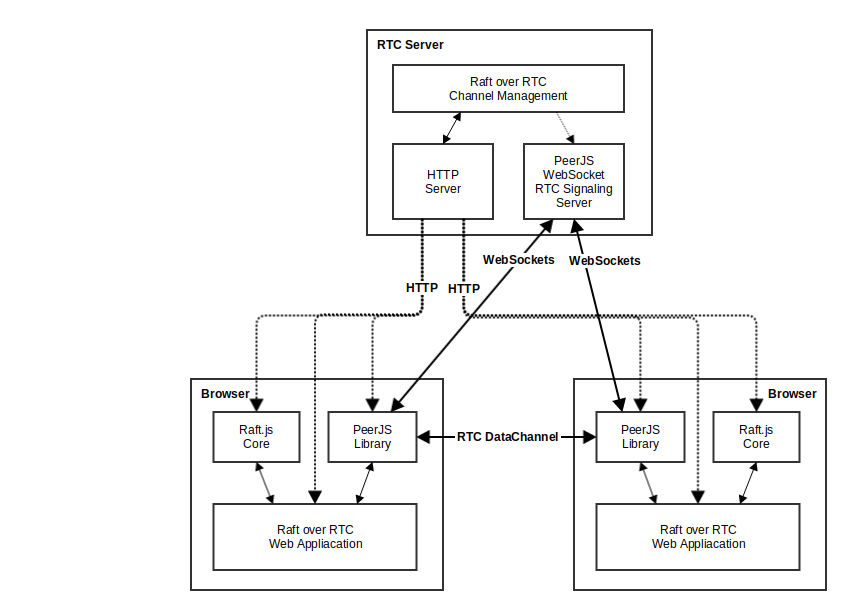
\includegraphics[width=15cm]{raft_rtc_architecture}}
\caption{Raft over RTC Architecture}
  \label{fig:raft_rtc_architecture}
\end{figure*}

\subsection{Incremental Steps}

During the planning phase, the project was broken down into ten incremental steps:

\begin{enumerate}
\item Simple WebRTC messaging: implement a small JavaScript application that uses the PeerJS client library and an unmodified PeerJS signaling server. Demonstrate communication over WebRTC DataChannel using two browser instances (or browser tabs).

\item Raft.js over WebRTC: combine the existing Raft.js implementation with the small JavaScript application above to demonstrate Raft over WebRTC. This step uses a statically configured three node cluster (three browser tabs). The PeerJS signaling server is polled to retrieve the list and other clients and the Raft cluster is started when the number of PeerJS clients reaches three.

\item Updated Raft.js: update the Raft.js implementation to match the latest description of the Raft protocol (as described in "Consensus", Ongaro dissertation). This includes the implementation of the simplified membership change algorithm (sequential changes) and the separation of the log commit and state machine apply concepts. [Additionally, the new Raft.js implementation always starts a new Raft cluster as a cluster with a single node and additional nodes are dynamically added to the cluster (as suggested in section 4.4 of the paper).]

\item Dynamic Raft.js over WebRTC: enhance the signaling server with support for sessions/channels to enable multiple separate Raft clusters. Start each cluster with a single node and automatically add and remove Raft nodes as they come and go.

\item Visual representation: display Raft node state and RPC statistics in addition to the internal Raft log messages.

\item Sessionless/Datagram RPC messages: extend Raft RPC requests and response messages so that RPC responses have enough context to be handled separately from RPC requests. Specifically this enables Raft to support a datagram (sessionless) network transport.

\item Atomic state machine operations: implement a state machine update operation that succeeds against the specified key only if no other operation has been applied to a key since the last time the client read from that key.

\item Automatic client request forwarding: extend the client request RPC to also be sessionless/datagram based. Implement a asynchronous JavaScript function that determines which node is the leader and forwards client request RPCs to the leader. This function must also correlate responses to the client request and invoke the callback for the original request.

\item Chat application: add the ability to send a message to the chat log using the client request forwarding functionality with an atomic state machine operation. Show the current chat history based on the chat entries in the state machine.

\item Server as Raft.js peer (aspirational): enable server nodes (Raft.js running on Node.js) to fully participate as Raft cluster nodes.
\end{enumerate}

Steps 1-9 were successfully implemented for this paper. Step 10 was an
aspirational goal because this functionality is not yet supported in
PeerJS although it is being tracked by issue report:
https://github.com/peers/peerjs/issues/103

\subsection{Server}

The file `rtc\_server.js` implements the signaling server for the Raft
over WebRTC application. The server extends the PeerJS
`ExpressPeerServer` object in order to provide WebRTC signaling. In
addition to the signaling function, the server also provides the
following service endpoints:

\begin{enumerate}
\item Static web service endpoint: this serves the static HTML, CSS and JavaScript that make up the Raft over WebRTC web application.

\item New channel endpoint: when a browser loads this endpoint, a new PeerJS channel is created and the browser is redirected to a URL for loading the main application (via static file service above).  The redirect URL has a query string appended that contains the channel ID. In addition the redirect URL has a fragment identifier (hash/history) that communicates to the web application that this is the first server in the channel.

\item Peer list endpoint: this endpoint takes a channel ID and returns the list of WebRTC peers (browser user agents) that are currently registered in that channel.

Refer to the "4.3 Client" section for a description of how these
endpoints interact.
\end{enumerate}

\subsection{Client}

\begin{figure*}[Ht]
\centerline{\includegraphics[width=15cm]{raft_rtc_sequence}}
\caption{Raft over RTC Sequence Diagram}
  \label{fig:raft_rtc_sequence}
\end{figure*}

The Raft over WebRTC testing application is designed as a single web
page (`rtc.html`). The application has different starting behavior
depending on the value of the URL query string (the URL component
following the "?" and up to the "\#") and the fragment identifier (the
URL component after the "\#").

When a new Raft cluster is created, the browser (user agent) connects
to the server new channel endpoint. This endpoint causes the server to
create a new channel for PeerJS signaling. Once this is complete the
server responds to the browser with a redirect message that contains
the new channel identifier in the query parameter and an indication
that this is the very first Raft cluster node in the fragment
identifier.

The browser follows the redirect and loads the static web application
at the static file endpoint provided by the server. This includes the
main application page (`rtc.html`), the core raft algorithm
(`base.js` and `local.js`), the PeerJS client library (`peer.js`), the
actual Raft over WebRTC implementation (`rtc.js`), and a layout
stylesheet (`web/demo.css`).

If the URL fragment identifier is set to "firstServer", then this Raft
node is initialized as the leader of a single node cluster and all
normal timers are started. The fragment identifier is then unset. The
query parameter contains the ID of this cluster (the PeerJS channel).

Subsequent nodes are added to the same Raft cluster by starting a new
browser context (separate browser, browser window, or browser tab) and
loading the same URL (which no longer has the "firstServer" fragment
identifier). There is a convenience link provided in the application
page that opens a new window with a new cluster node.

When the page first loads, a PeerJS signaling connection is
established with the server. Once this connection is established, the
application will be notified when any PeerJS clients connect to or
disconnect from the server. After the PeerJS signaling connection is
established, the client immediately queries the Peer list endpoint to
discover any clients that were connected prior to when this node
connected to the server.

The web application also begins a periodic async polling function
(`addRemoveServersAsync`) when the page loads. When the node is a Raft
leader, the function compares the current active list of PeerJS clients to
the Raft cluster node list. If there are any differences between the
two lists, then any new clients are added to the Raft cluster and
missing clients are removed from the Raft cluster one at a time using
the `addServer` and `removeServer` RPC calls. Servers additions are
prioritized before removals (as recommended in Ongaro 4.4 TODO/CITE)
in order to maximize availability.

When an instance of the web application starts that is not
a "firstServer", the normal Raft timers are not automatically enabled
until the server receives an RPC. The prevents the server from
possibly becoming a leader before it is incorporated into the cluster
by an appendEntries RPC from the "true" leader.

In addition to the low level Raft message log, the following
statistics are shown in the application:

\begin{enumerate}
\item \emph{Term}: the current Raft leadership term.
\item \emph{State}: the current Raft node state (follower, candidate, or leader)
\item \emph{Cluster Size}: a count of the current Raft cluster membership (number of nodes currently participating in the cluster)
\item \emph{Log Length}: number of entries in the transaction log.
\item \emph{Request Votes Sent/Received}: the number of `requestVote` RPCs that have been sent from and received by this node.
\item \emph{Append Entries Sent/Received}: the number of `appendEntries` RPCs that have been sent from and received by this node.
\end{enumerate}

\section{Results}

\subsection{Manual Testing}

\subsubsection{Setup}

The initial way that the application was tested was by loading the
initial landing page to create a Raft over WebRTC cluster with
a single leader. Here is a screenshot of the browser after the first
node is created:

\begin{figure*}[Ht]
\centerline{\includegraphics[width=15cm]{browser_1}}
\caption{Raft over WebRTC Browser with One Node}
  \label{fig:browser_1}
\end{figure*}

Then four more Raft nodes were then added to the cluster by clicking
on the embedded "create a node" link in the application. Here is
a screenshot of the browser once four new nodes are added to the
cluster (5 total):

\begin{figure*}[Ht]
\centerline{\includegraphics[width=15cm]{browser_2}}
\caption{Raft over WebRTC Browser with Five Node}
  \label{fig:browser_2}
\end{figure*}

After every change was made to the cluster all the nodes were checked
to ensure that the following steady state properties were observed:
\begin{enumerate}
\item only a single leader
\item all nodes have the same term and transaction log count
\item all non-leader nodes are receiving `appendEntries` RPCs from the leader
\item all nodes have the same perception of the cluster size
\item the transaction log entries are identical on all nodes
\item the state machine is identical on all nodes
\end{enumerate}

The current leader was then terminated. The other nodes were checked
for the steady state properties. This was repeated until only two
nodes remained in the cluster.

After the five node cluster was brought up, state machine commands
were manually sent to leader to add to the transaction log. This was
done using the JavaScript console as there is not yet a way to do this
via the interface. Again the nodes were checked for the steady state
properties.

Then the application was tested was by loading the initial cluster
creation landing page in a browser tab. Then nodes were randomly added
to the cluster (by clicking on the link embedded in the page) or
removed from the cluster (by closing a tab). After each change the
steady state properties were checked.

Similar testing to the above was done with browser instances on two
separate computers. In addition, cross-browser functionality was
verified by running nodes from the same cluster running simultaneously
in Chrome 42 and Firefox 37.


\subsubsection{Outcome}

The results of the manual testing above showed that Raft over WebRTC
was able to perform leader elections correctly, the log and state
machine was replicated correctly to all nodes, and the safety
properties were maintained. During testing the membership of the
cluster was changed numerous times (both node additions and removals)
and the Raft properties were maintained throughout. In addition,
client interaction was tested although the application does not
provide a friendly interface for doing so.

One limitation of the system is that the if the cluster membership
drops from two nodes to one node then the cluster will become
unavailable without manual intervention. This is because when there
are two nodes in the cluster, both nodes are required for for
a majority vote and when one member is forcible shutdown then the
remaining cluster node will be unable to commit transaction entries
and the cluster will become unavailable. There are several options to
get around this problem:

\begin{enumerate}
\item The node can ask the leader to be removed and then wait for the
  transaction to become effective before it disconnects.  This may not
  always be an option especially in a browser context where the user
  may immediately kill the window/tab without giving the application
  a change to remove itself from the cluster.
\item The signaling server can serve as a tie-breaker. This would allow
  the remaining leader successfully commit the removal of the other
  node. In the case of a partition, the signaling server must only
  vote for one of the nodes.
\item The node with the lower ID could have an implicit tie-breaker vote.
  This would allow one node of the partition to continue in the case
  of a network partition. If a node dies or is killed, this would only
  allow the cluster to continue to operate if the node that dies
  happens to have the higher ID.
\item The system could allow manual user intervention. However, this is
  only likely to work correctly in the case where the user of the last
  remaining node can be certain that the other node will never return
  otherwise they is the risk of data-corruption.
\end{enumerate}

Running a Raft cluster in a browser context leads to some level of
timer instability. The JavaScript execution context is a fully event
driven environment with a single thread of execution for a given
JavaScript context. JavaScript code is run when browser (or Node.js)
events trigger JavaScript code that is registered to that event. In
order to implement logic that runs periodically, JavaScript code
is register as a callback timer using the setTimer, setInterval or
requestAnimationFrame APIs. However, none of these mechanisms is
a precise timer. When a timer fires, the callback code they refer to
is added to the JavaScript event queue and events on the queue are
processed in the order they arrive. This means callbacks may be
delayed by other code that is already running or queued first.

However, there is another browser mechanism that is less well known
but that causes even larger delays in timer code execution. Modern
browsers often have dozens or even hundreds of windows and/or tabs
open simultaneously. In order to reduce CPU load, increase user
responsiveness and improve battery life, most modern browsers will
throttle the JavaScript callback timers for all windows and tabs that
are hidden or have not been directly interacted with for some period
of time. This throttling can cause timers to slow down by an order of
magnitude or more.

In the context of Raft over WebRTC, the slowdown of background page
timers means that whenever the leader node is residing on a page that
is in the background, the propagation of transaction log entries slows
down substantially. This also means that other nodes which are in the
foreground are more likely to have an election timeout timer fire and
they are more likely to become a leader because they are more likely
to be able to send and receive votes quickly than nodes that are in
the background. In this sense the problem is self-correcting because
over the long term because higher performing nodes more are likely to
start and win elections. This also indicates dynamic adjustment of
timeout values may be a fruitful area of further study.

\subsection{Automated Testing}

\subsubsection{Setup}

TODO: Setup for the automated tests. Description of SlimerJS. Creation of SlimerJS test scripts using JavaScript.

\subsubsection{Outcome}

TODO: Outcome of the automated tests.

The following figure shows the amount of time that the cluster takes to
elect a leader and then reconfigure the cluster to the the final size
(adding one node a time).

\begin{tikzpicture}
    \begin{axis}[
            title=Initial Cluster Activation,
            xlabel={Nodes},
            ylabel={Time (seconds)},
            grid=major,
        ]
        \addplot table {data/data_cluster_up.dat};
    \end{axis}
\end{tikzpicture}

The following figure shows the amount of time that a stable cluster takes to
propagate, commit and apply a single state machine change to the state
machines on every cluster node.

\begin{tikzpicture}
    \begin{axis}[
            title=Message Propagation,
            xlabel={Nodes},
            ylabel={Time (ms)},
            grid=major,
        ]
        \addplot table {data/data_propagate.dat};
    \end{axis}
\end{tikzpicture}

The following figure shows the amount of time that it takes for
a stable cluster to recover (elect a new leader and remove the failed
servers from the cluster) when one or more nodes fails. The first line
shows the recovery time when just the leader fails. The second line
show the recovery time when one less than half of the nodes fail.

\begin{tikzpicture}
    \begin{axis}[
            title=Node Failure Recovery,
            xlabel={Nodes},
            ylabel={Time (seconds)},
            grid=major,
            legend entries={$Leader Down$,$Half Cluster Down$},
        ]
        \addplot table {data/data_kill_leader.dat};
        \addplot table {data/data_kill_half.dat};
    \end{axis}
\end{tikzpicture}



\section{Next Steps}

One of the useful outcomes of this project was that it brought to
light many areas where further study of Raft, WebRTC, and Raft over
WebRTC should be pursued.

Here are some interesting areas for further exploration:

\begin{enumerate}
\item Explore the use of alternate WebRTC transport modes for relaxing
  ordering constraints and delivery guarantees. Since the Raft
  protocol is tolerant of out-of-order and dropped messages, it is
  possible that Raft over WebRTC could be more efficient with these
  one or both of these constraints relaxed.
\item Test the survivability of the cluster when the signaling server is
  becomes completely unresponsive or just very slow.
\item Explore models for dynamically adjusting Raft timeout values to
  account for changing network and browser conditions.
\item Test the ability of the system to catch up stale nodes by
  disconnecting one or more nodes, run the cluster for some period
  time with transactions created periodically, and then reconnect the stale
  clients.
\item Implement a user interface for sending commands to the transaction
  log and for viewing the current state of the Raft state machine.
\item Explore models for dealing with the case where the cluster goes from
  two nodes down to one node. Can usefulness and availability be
  improved without sacrificing Raft safety constraints.
\item Test the system in more various network environments. Determine the
  reliability of establishing direct browser-to-browser communication.
  Determine if corporate firewalls make this as difficult as is
  implied in some of the documentation and standards texts.
\item Implement and test forwarding client requests rather than default
  redirecting the client to the leader. In other words, allow client
  requests to originate from any node of the cluster and be redirected
  automatically to the leader (rather than the current manual
  process).
\item Perform quantitative and real-world testing to better characterize
  the performance, availability and scalability characteristics of the
  system.
\item Explore models for timing out and automatically removing nodes
  when they become unresponsive without needing to be notified by the
  signaling server that the nodes have disconnected.
\item Test larger scale deployments across multiple systems. Determine the
  factors that affect scalability and characterize scaling limits.
\item Perform wider cross-browser testing including Internet Explorer and
  Opera.
\item Implement Raft log compaction.
\item Explore models that allow for a combination of strict shared state
  and high performance bulk data such as media or object blobs. For
  example, the data with full consensus might contain hashes that to
  the refer to bulk data.
\item Implement a Node.js based Raft over WebRTC application. This would
  allow non-browser contexts to participate in the Raft cluster
  together with the browser clients. PeerJS issue
  [103](https://github.com/peers/peerjs/issues/103) must be resolved
  for this to be feasible.
\item Explore a design where some nodes of the cluster are non-voting and
  are not counted as part of transaction commit quorum. However, these
  nodes would still be included in the log replication algorithm. One
  model this would enable would be a configuration where a small group
  of voting nodes serve as the hub for a larger group of non-voting
  nodes. This may enable higher scaling of the system. It also enables
  interesting applications such as a logging or backup nodes.
\end{enumerate}


\begin{acks}
I would like to thank my academic supervisor, David Levine, for his
excellent input and oversight of this project. I would also like to
thank Diego Ongaro for his amazing work on the Raft protocol and paper
which made implementing a Raft implementation a pleasure. There are
too many people involved in the creation and standardization of WebRTC
but I would like to thank them for their tireless work to make
browser-to-browser communication possible. Last but not least, I would
like to thank my family for putting up with the long nights and
weekends I spent on this project. Thanks!
\end{acks}


% Bibliography
\bibliographystyle{ACM-Reference-Format-Journals}
% TODO: references
\bibliography{acmtog-sample-bibfile}
                                % Sample .bib file with references that match those in
                                % the 'Specifications Document (V1.5)' as well containing
                                % 'legacy' bibs and bibs with 'alternate codings'.
                                % Gerry Murray - March 2012

%\received{September 2008}{March 2009}

\end{document}
% End of v2-acmtog-sample.tex (March 2012) - Gerry Murray, ACM
